\documentclass[11pt, english]{../Template/NTNUoving}
\usepackage[utf8]{inputenc}
\usepackage[T1]{fontenc}
\usepackage{float}
\usepackage{enumitem}
\usepackage{csquotes}
\usepackage{algorithm}
\usepackage{algorithmic}
\usepackage{listings}
\usepackage{listings}
\usepackage{color}
\usepackage{biblatex}
\usepackage{hyperref}
\usepackage{pdfpages}

\addbibresource{references.bib}
\ovingnr{4}    % Nummer på innlevering
\semester{Spring 2021}
\fag{Methods in Artificial Intelligence \\ TDT4171}
\institutt{Department for Computer Science}

\begin{document}

\textit{Note: The graphs when using multiple attributes were pretty hard to fit, but the resolution should be high enough so you can zoom in to see the numbers/names.
If this is not the case these pdfs with the graphs are also uploaded on BB.}


\begin{oppgave}

    The TA can test the different cases by changing the variable \texttt{continuous\_variables} to decide which attributes should be treated as continuous variables and commenting/commenting out
    which attributes to remove or add.

    \begin{punkt}
        The continuous variables are $Age$, $Name$, $Ticket$, $Cabin$, $Fare$ as these are pretty much
        unique for almost all (except for $Cabin$ where more people can live in same cabin, but this does not warrant enough discrete cases to make it discrete). Both $SibSp$ and $Parch$ can be treated as
        both as for most persons this number should be somewhere between 0-10. However, there are edge cases and this is in reality a continuous variable. This means that when we train it
        with these as discrete attributes there is a chance that the DT meets a unhandled case (for example $SibSp = 11$) when used on testing data.
        In my DT model I have handled this by making an educating guess if $Parch$ or $SibSp$ are chosen as discrete attributes and there is no known case of this from the
        training data.

        When trained on all discrete attributes (with $SibSp$ and $Parch$) these were the results:
        
\includepdf[pages=-]{graph1.pdf}

        This model is extremely complicated and got an accuracy of 86.8\%. It is very likely that this is an overfitted model.
        The attribute $Embarked$ shouldn't really affect the survival of the passenger so I decided to drop this. The results:
        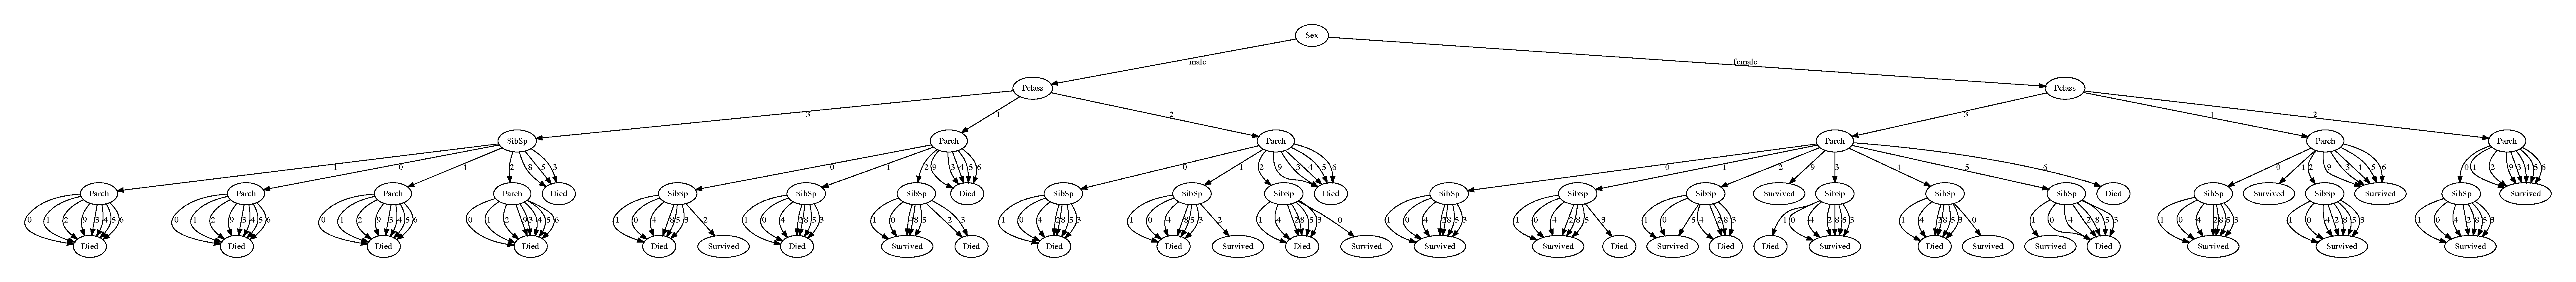
\includepdf[pages=-]{graph2.pdf}

        The graph got a bit simpler and the accuracy increased to 88.0\%, this makes sense because
        the attribute $Embarked$ was overfitting the problem.

        In fact the best results are gotten by also removing the $Parch$ attribute:
        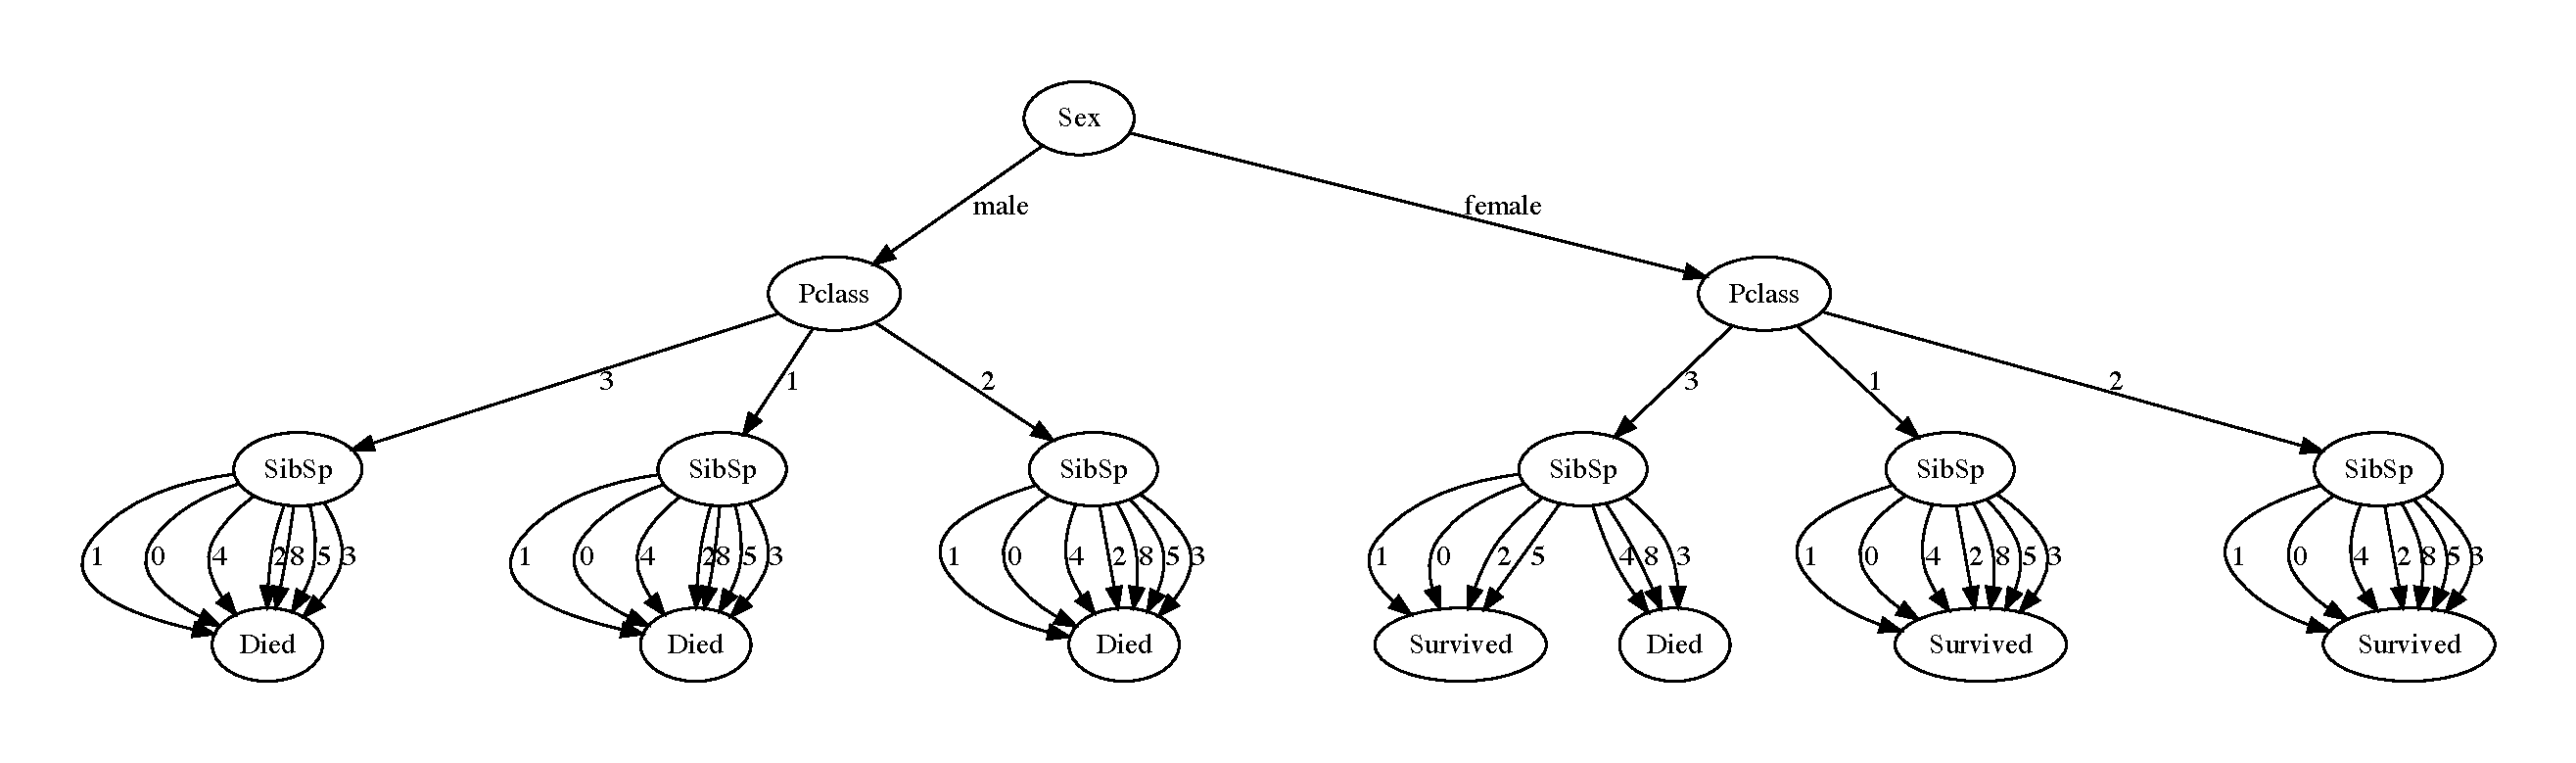
\includepdf[pages=-]{graph3.pdf}

        The graph is now easily readable and the accuracy improved to 88.5\%.

    \end{punkt}

    \begin{punkt}
        Support for continuous variables were added by changing the $gain$ function to
        loop over the unique values of the continuous attribute and then find the best split point (taken by averaging between two points).

        $Age$ and $Cabin$ was removed since they had some missing values. $Ticket$ was removed as the ticket number itself should not have
        any influence on survival, and it is also not an easy value to split on as it has a combination of string and int which would need more processing.

        The results by using the attributes $Fare$, $Parch$ and $SibSp$ as continuous attributes with the discrete values $Sex$ and $Pclass$:
        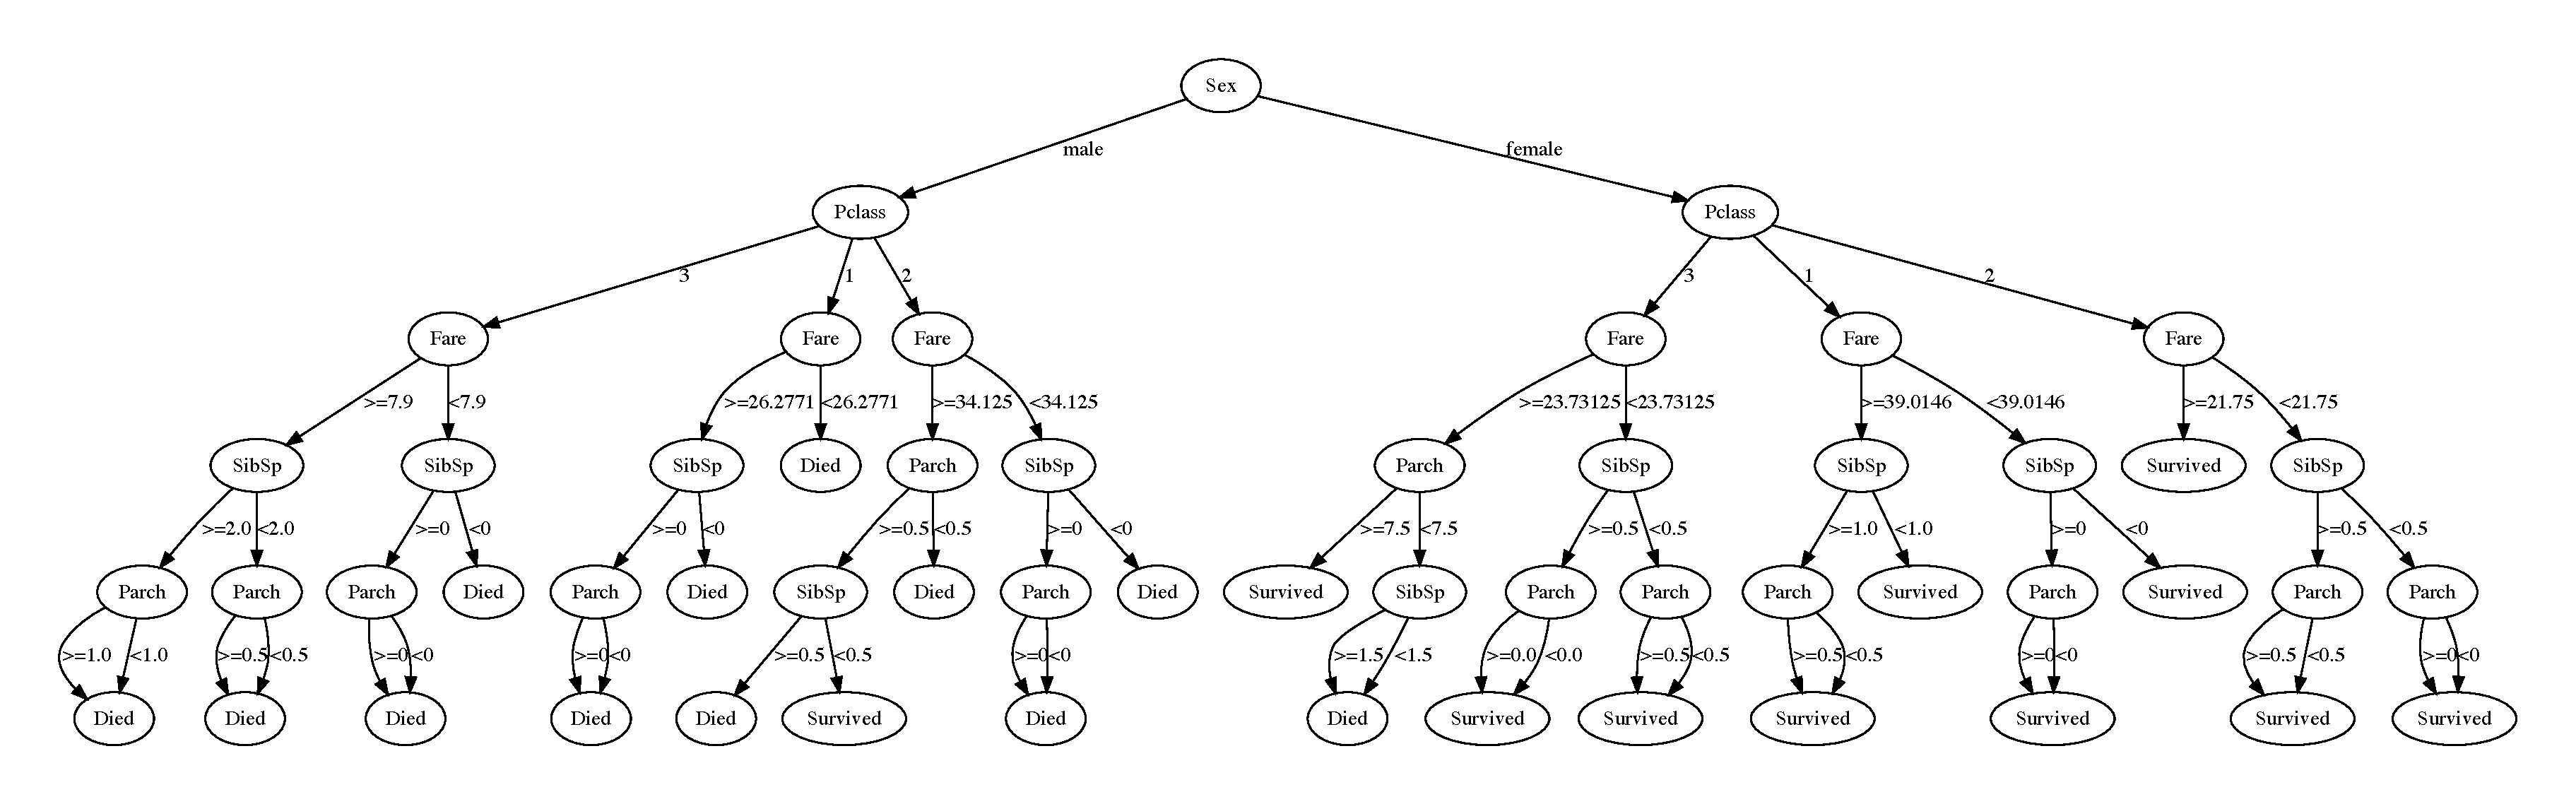
\includepdf[pages=-]{graph4.pdf}

        The accuracy was also 88.5\% which is the same as the best results using discrete attributes only. To achieve this we had to remove $Parch$ in the discrete case,
        this means that the DT in \textbf{a)} was overfitting the problem when using $Parch$ as an discrete value.
        There is an argument to be made for whether $Fare$ actually should influence survival, but in this case the results would have been the same (88.5\% accuracy on test set).
    \end{punkt}

    \begin{punkt}
        The best performance in both \textbf{a)} and \textbf{b)} was equal at 88.5\%. Although we could expect better results when also using
        continuous values this was not the case, however a significant gain is that the DT is much simpler and although it is more heavy to train as atleast my algorithm goes
        through all distinct continuous values and checks the split gain. In this case the expected performance did not increase so it does not warrant the usage of continuous values.

        Another interesting aspect would have been the $Age$ attribute because of the women and children first
        code of conduct when saving passengers on the Titanic\cite{women}. Since there was a lot of missing values in the training data set we did not use this attribute, but it could have increased performance.

        There are several methods we could have used to improve this simple DT:
        \begin{enumerate}
            \item \textbf{Bootstrapping}: With trainingsets which are this small (small in the machine learning world) there can be a lot of variance when training on different data.
            For example if we were to split the trainingset in two halves and then train a DT on each one we could get two trees with fairly different results (high variance). In order to
            combat this we could use Bootstrapping\cite{ml}\cite{bootstrapping}. The idea is to minizime the variance by
            using sub-samples of our trainingset with replacement and train several DTs on these sub-sample trainingsets. The key is that we don't use just one of the trees when predicting, but we calculate the
            \textit{average} over all the DTs, which will reduce the overall variance and could give better accuracy.
            \item \textbf{$\chi^2$-pruning}: Unless we remove some of the irrelevant attributes by hand there is a general problem of overfitting with our DT. For example when using the attribute $Embarked$ which should have no bearing
            on survival. To combat this we could use a technique called $\chi^2$-pruning. This pruning removes irrelevant nodes, the key here is to determining the relevance of a node.
            This can be done by finding nodes that have close to 0 in information gain, however underlying noise can influence this, so we will also use a significance test of for example 5\% deviation from 0.
            We can then replace these irrelevant nodes with leaf nodes and severly simplify the tree which combats overfitting and requires less domain knowledge by the person who writes the DT.
            \item \textbf{Gain ratios on multivalued attributes}: The information gain test we are using in this DT can be misleading when using it on multivalued attributes such as $Pclass$, $Parch$ etc.
            In the extreme cases for example when $SibSp$ has very few cases on each variable, this would result in a high information gain, but it would not necessarily give us the best tree. To combat this we could
            use gain ratio \cite{gain} which takes this into account. This could possibly lead to a better tree because the splits would be chosen on a more equal basis among different
            attributes with different number of possible values.
        \end{enumerate}
    \end{punkt}
\end{oppgave}

\begin{oppgave}

    The columns missing data are the $Age$ and $Cabin$ columns.
    $Age$ is just an integer, but $Cabin$ can be a combination of several
    string and integers, for example "C32 C31", which makes this attribute harder to replace.

    Both of these are regarded as continuous variables, which means in order to replace them we should use some sort of
    regression imputation rather than classification (it would be possible to use classification, but it does not make as much sense).

    These are the proposed solutions:

    \begin{enumerate}

        \item \textbf{k-Nearest-Neighbors}\cite{knn}: This method relies on finding the nearest neighbors of the rows with missing values by averaging over them. The hard thing here is to find a good distance metric.
        This is how I see the implementation:
        \begin{enumerate}[label=\arabic*]
            \item Calculate the distance metric, for discrete attributes and the continuous attributes $Name$, $Cabin$ I would use the Hamming distance \cite{hamming}. For the continuous attributes $Fare$, $Ticket$ and $Age$ I would use the Euclidean or Cosine distance between them.
            \item Find the $k$ nearest neighbors (design parameter), average over these to choose the continuous output on $Age$ and $Cabin$.
        \end{enumerate}
        \textbf{Advantages}:
        \begin{itemize}
            \item Non-parametric, does not rely on parameters like for example mean or variance
            \item Simple to implement, we only need to worry about the distance metric which could be hard, but managable.
        \end{itemize}
        \textbf{Weaknesses}:
        \begin{itemize}
            \item Very expensive as it has to go through the whole dataset in order to find the nearest neighbors, however we have a smaller trainingset and not too many attributes so my guess is that it wouldn't be too expensive.
            High dimensions (number of attributes) and large datasets are the big drawback of this method.
            \item Can be sensitive to noise in the dataset, we may need to manually remove outliers.
            \item Requires high domain knowledge to find good distance metrics.
        \end{itemize}
        This method assumes that the distance metrics are good enough, which is hard to determine before testing with it.

        \item \textbf{Mean Imputation}\cite{mean}: A single imputation method which works by imputating a variable with the mean of that variable.
        This is how I see the implementation:
        \begin{enumerate}[label=\arabic*]
            \item Calculate the mean of the variable, for $Age$ this is straight forward, but $Cabin$ requires a bit more thought. A simple method is to just
            take the mean of the character (A, B, C etc.) and the mean of the integer part and then combine these, this will however not take into account the possibility of living in multiple cabins.
            This can be solved by for example by taking the mean of number of cabins and then choose the second cabin nearby of the first.
            \item Assign the missing values with this imputated mean.
        \end{enumerate}
        \textbf{Advantages}:
        \begin{itemize}
            \item Very simple to implement, requires little calculation.
            \item Does not change the mean of the variable.
            \item Requires no domain knowledge to implement and use.
        \end{itemize}
        \textbf{Weaknesses}:
        \begin{itemize}
            \item This very simplistic way of viewing the data can attenuate any underlying correlations with other variables as it just chooses based on mean.
            \item Parametric; relies and make assumptions on mean, which we can't confirm are correct.
        \end{itemize}
        Assumes that the mean is representative and assumes that the variable has no correlation with the other attributes, which in this case I would say is wrong
        as for example $Cabin$ correlates with the $Cabin$ of people with same name (families are more likely to live in the same or nearby cabins).
        I do not believe this method should be chosen for filling out these missing values.

        \item \textbf{Multiple Imputation}\cite{MI}: This is a method which averages the outcome across multiple imputated datasets to deal with the issue of increased noise when imputating.
        This is how I see the implementation:
        \begin{enumerate}[label=\arabic*]
            \item Draw $m$ imputated values from a distribution (create normal distribution for variable) until there are $m$ completed datasets. Here one could also use MCMC (Markov Chain Monte Carlo) \cite{MCMC} to draw th $m$ imputated variables.
            \item Analyze the $m$ datasets using a complete data method, returning $m$ analysises.
            \item Pool the $m$ analysis into one result. This is done by calculating parameters such as mean, variance and confidence interval. The values are then imputated from this distribution.
        \end{enumerate}
        \textbf{Advantages}:
        \begin{itemize}
            \item Easy to implement (although harder than the previous method).
            \item The problem with single imputation (such as mean imputation) is the negligence of uncertainty. This leads to overly precise results and errors in the imputated values.
            Multiple imputation combats this problem by doing the imputation several times and combining the results, this leads to no biases if the imputation model is correct.
        \end{itemize}
        \textbf{Weaknesses}:
        \begin{itemize}
            \item Can lead to errors if the imputation model is incorrect.
            \item Slightly more advanced (and therefore harder to implement) than the previous methods.
            \item More expensive calculations (drawing, analyzing and pooling) than single imputation methods.
            \item Parametric; relies and make assumptions on parameters like mean and variance which we can't confirm are correct.
        \end{itemize}
        This method is very dependent on the imputation model chosen, which can also be its downfall. However it should still be more accurate than the
        single imputation methods like mean imputation. This is generally the best method for imputation and I would have used this.
    \end{enumerate}
\end{oppgave}

\printbibliography
\end{document}
